\documentclass[a4paper,twocolumn]{article}
\usepackage[utf8]{inputenc}
\usepackage{url}
\usepackage{graphicx}

% This assignment requires you to write an essay on Software Engineering for
% AI/AS ("AI Engineering"), how it relates to your research, and how you can
% apply SE principles and tools in your project / on your sub-topic. Please only
% use diagrams/illustrations if necessary, and do not count these towards the
% length of the essay. The essay should be a minimum of 3.5 A4 pages in length,
% and a maximum of 5 A4 pages in length, excluding references. The font should
% be Times New Roman (or equivalent) and 11 point. Be sensible in formatting /
% layout choices.

% The essay should be structured as follows:

% 1. Begin with an introduction/abstract to your research and topic area. This
%    should be a maximum of 400 words, and should provide (just) enough basis so
%    that your answers to the questions below can be understood.

% 2. Select at least 2 principles/ideas/concepts/techniques from Robert's
%    lectures and discuss how they relate to your research and topic area.

% 3. Select at least 2 principles/ideas/concepts/techniques from the guest
%    lectures and discuss how they relate to your research and topic area.

\newcommand{\Section}[1]{Section~\ref{#1}}
\newcommand{\Figure}[1]{Figure~\ref{#1}}
\newcommand{\Table}[1]{Table~\ref{#1}}
\newcommand{\Appendix}[1]{Appendix~\ref{#1}}

\begin{document}

\title{Behavioral Software Engineering for Code Review Tools\\
\large WASP Software Engineering Assignment} \author{\small Lo Heander,
\texttt{\small lo.heander@cs.lth.se}}
\date{}

\maketitle

\section{Introduction}

The DAPPER project's goal is to answer the research question \textbf{``how can
code reviews be made fit for purpose?''}, which is a question that is more and
more relevant today with more and more of software development being done
remotely to some degree. The advent of AI-supported development tools like
Copilot\cite{bird_taking_2023} and ChatGPT\cite{sobania_analysis_2023} also
shifts the focus for developers even more from writing new code to reviewing
code and integrating it into their code bases. 

Code review is a task with a high cognitive
load\cite{pascarella_information_2018}, requiring the reviewer to focus, hold
the code in their memory, look for problems and connections, keep the goal of
the merge request in mind and also take decisions around writing comments and
approving or rejecting the merge request. This limits how long a developer can
keep doing code reviews and how many they can complete before they are fatigued
and the benefits decrease. 

Despite these problems, code review tools have changed surprisingly little since
the first software tool for code view, ICICLE\cite{brothers_icicle_1990}, was
introduced over three decades ago. More modern tools have colored diff-views and
run in the browser, but ICICLE already had many of the core features such as the
central diff view, the ability to add comments, support for annotations by
static analyzers and support for working in a distributed network environment.
This, I think, indicates a superlativist
assumption\cite{green1991comprehensibility} where one tool is assumed to be the
best regardless of context. It favors certain kinds of software development, for
example writing code over UI prototyping and promotes a file-centric view with a
lexical diff over looking at code changes through the lens of exported APIs,
inheritance structures or execution flow. 

To explore these goals and the research question I use an interdisciplinary
approach combining computer science with methods from sociology and psychology
such as ethnography\cite{h_sharp_role_2016}, grounded
theory\cite{adolph_using_2011} and distributed
cognition\cite{hutchins1995cognition}. I believe that to find the answers here,
the practices, tools, interactions and patterns \emph{needs} to be observed from
an interdisciplinary perspective to raise the perspective to a higher level. To
observe the effects and the outcomes and acknowledge that these systems work in
interaction with a team and with their process for version control, continuous
integration, code review, code merging, deployment and maintenance. 

\section{Software Engineering principles from lectures}

\subsection{Behavioral Software Engineering}

The core perspective of Behavioral Software Engineering is to focus on the
people involved in developing, maintaining, using, specifying, deploying and
testing software systems. The argument is that since these people are human and
not rational, focusing on the technical aspects or the process is not enough.
The individuals, groups and organizations needs to be an important factor in how
the systems are engineered and having this as the main focus can be at least as
effective as focusing on the technology if not more so.

This brings in many ideas and concepts from psychology into the software
engineering field. A key figure in this movement is Professor Daniel Kahneman
who have made important contributions within the theories of loss aversion,
prospect theory, hedonic psychology and more. While Kahneman applied these
theories mainly to economics, they have a reflection in the behavior of the
people involved also in software engineering. By better understanding the humans
involved, we can better understand the dynamics and motivations that drive
software projects to succeed or fail.

These aspects are central to my research on trying to make the specific software
process of code review fit for the humans involved in it. To find and understand
the effects of both the code review process and the tools used on software
quality, software teams and collaboration within an organization the focus must
be on the humans involved. This, I believe, is best studied using methods from
the social sciences and psychology in order to understand the tools and
processes not just as a list of features but as a cause and effect relationship
on the individuals and their organizations.

\subsection{Quality Assurance in Software Engineering}

In the lecture about Quality Assurance in Software Engineering, Robert Feldt
starts by introducing the difference between Verification and Validation.
Verification is checking whether we are building the product right and can be
acheived for example through automated software testing and code reviews.
Validation on the other hand is about checking whether we are building the right
product, which brings us into the domain of Requirements Engineering. 

To validate a system we must ensure that the system fulfills a real need and is
possible to be deployed, maintained and used successfully. For ML-systems, this
will often extend to also validate the input data used for training and
benchmarks and make sure that it is representative and corrected for biases that
could make the system have undesired unfairness or poor performance.

For efficient verification, one technique stood out as particularily interesting
to me: Property-based Testing. The idea is to combine invariant parameterised
properties of a system with generation of random test data. This makes it
possible to express the expected behavior in a compact way that is easy to
understand, and still create and test thousands of test cases to be able to find
corner cases where the expected properties break. In for example autonomous
driving, I have seen this combined with machine-learning algorithms that try to
predict the most tricky data possible and generate a higher density of random
values around these boundaries to really challenge the system and improve its
robustness~\cite{Song2024}. 

\section{Software Engineering principles from guest lectures}

\subsection{Levels of assistance and automation}
\label{sec:lenberg}

Per Lenberg held a very interesting guest lecture explaining why Behavioral
Software Engineering was especially interesting and necessary to create and
maintain the complex systems built by SAAB Air Trafic Management. He highlighted
how organizational charts may look simple and heirarchical, but in practice they
are full of hidden interpersonal connections that are what truly defines how the
organization behaves. 

\begin{figure}[h]
    \centering
    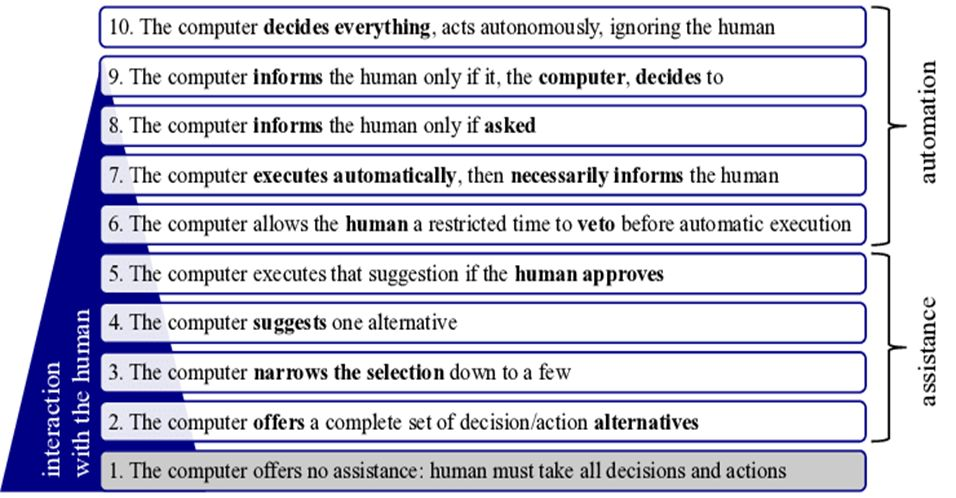
\includegraphics[width=0.9\columnwidth]{automation_levels.png}
    \caption{Automation levels by Per Lenberg}
    \label{fig:alevels}
\end{figure}

Lenberg also talked about automation levels (figure \ref{fig:alevels}), ranging from
level 1 where the computer does nothing at all up to level 10 where the computer
takes and executes all decisions without involving the humans at all. It is an
interesting discussion both what level of automation that is desired and safe
for an application such as Air Trafic Management, but also applied to something
like code review, testing and software engineering.

\subsection{System Verification using AI-based systems}

Dhasarathy Parthasarathy from Volvo introduced how they used an AI-based system
to generate new test cases for system verification. They used large language
models to analyze the documentation and system specifications across the
different subsystems involved in the operation of a truck and translate for
example different API-names and constants and then automatically write test
cases.

I do find the approach a bit odd. In an environment that is already very complex
and safety critical, such as for a truck driving on the highway during a
long-haul delivery, it seems counter-intuitive to introduce another complex
system that is even harder to explain and verify. If there are systematic faults
or misunderstandings in the tests generated that don't cause the tests to fail
but rather to enforce unwanted behavior, how will that be discovered? How can
the test generation system be re-trained to correct for this? In many ways, it
ties into the discussions raised under Lenberg's lecture
(section \ref{sec:lenberg}): what level of automation is appropriate, safe and
desired for which tasks?

\section{Related work}

% 4. Find two full/long papers published in one of the CAIN conferences (3 have
%    been held so far, all linked from
%    https://conf.researchr.org/series/cainLinks to an external site.), download
%    and read them and then write in your assignment, for each paper: a,
%    Describe the core idea(s) of the paper and why it/they are important to the
%    engineering of AI systems b, How the paper relates to your own research c,
%    How your research and its results would fit into a larger AI-intensive
%    software project where one of the core ideas from the paper would benefit
%    the project if applied. Describe both how the paper could help improve the
%    project and how your WASP research would fit into the project. d, Discuss
%    briefly how your research could be potentially adapted/changed to make AI
%    engineering in the project based on the idea of the paper even
%    better/easier.
% 
% Your answers to question 4 is the main part of your essay and should be
% approximately 2 A4 pages in length, 1 page per paper.

\subsection{Design Patterns for AI-based Systems}

``Design Patterns'' is a concept in Software Engineering that describes and
names proven and reusable solutions to frequently occuring
problems~\cite{Gamma2001}. In my first chosen research paper, Heiland et
al.~\cite{heiland_design_2023} presents an multivocal literature review over both traditional
Software Engineering Design Patterns that are applicable to AI-based system, as
well as new emerging patterns that are unique to, or more relevant to, these
systems. The authors motivation for the study is that since there are
indications that design patterns improves the overall software quality, they are
likely to give similar effects on system quality for AI-based systems as well.
Having a comprehensive overview over possible patterns will help both in future
research of this as well as when implementing and refactoring AI-based systems.

Heiland et al. finds 70 design patterns described both in academic and
practitioner literature. Roughly half of these, 34 patterns, are specific to
AI-based system while the rest are applicable to both AI-based system and
traditional software systems. An interesting finding is that these categories of
patterns address different areas of the system quality. Traditional design
patterns are applied predominately to improve process and implementation aspects
while new AI-system-specific patterns focus on improving security, safety and
deployment aspects. The authors see this as an argument in the debate around if
there is a need for a new field of ML Engineering distinct from Software
Engineering. If around half of the patterns are specific to AI-based systems and
also address aspects unique to this domain, that is an indicator on
the differences between traditional software systems and AI-based systems are
large enough to merit their own research fields and professional disciplines.

Techniques and best practices to improve system quality is closely related to my
research field. Because code review in itself is (among other things) a quality
assurance tool, identifying proven design patterns in the code under review
could help the reviewers understand and critique the code. In the paper, Heiland
et al. presents a web-based application they developed to make the patterns
accessible and easily
browsable\footnote{\url{https://swe4ai.github.io/ai-patterns/}}. 
Through this app, the design patterns are stored and described in a
machine-readable JSON format. This could assist in building tools that both
gives developers access to this database during code reviews or automatically
tries to identify and mark out the patterns in the code under review.

Further, my research project also aims to propose improvements in code review
tools that address the shortcomings and frictions found by both other
researchers and in my initial studies. One important avenue to explore here is
how to leverage AI-based system to assist software developers before,
during and after code reviews. To make these systems perform well it would make
sense to use established design patterns for both implementation, architecture,
security, and so on.

\subsection{SOLID Design Principles Applied to Machine Learning Code}

SOLID design principles are principles for improving the design of
object-oriented software~\cite{Martin2009} that are well-know and widely applied
in the industry. In my second chosen CAIN research paper Cabral et
al.~\cite{Cabral2024} studies if applying these principles also improves code
understanding of Machine Learning code. 

\bibliography{references.bib}
\bibliographystyle{ieeetr}

\end{document}
